% -------------------------------------------------------------------
% Area de importação de pacotes do Latex
% -------------------------------------------------------------------

\documentclass[a4paper,12pt]{article}
\usepackage[english,brazilian]{babel}
\usepackage[utf8x]{inputenc}

\usepackage[a4paper,left=30mm,right=20mm,top=30mm,bottom=20mm,includehead,includefoot]{geometry}

\usepackage{setspace}
\onehalfspacing %% 1,5-spacing

\usepackage{graphicx}
\graphicspath{ {../codigos/imgs/} }
\usepackage{subcaption}

\usepackage{amsmath}

% Default fixed font does not support bold face
\DeclareFixedFont{\ttb}{T1}{txtt}{bx}{n}{10} % for bold
\DeclareFixedFont{\ttm}{T1}{txtt}{m}{n}{10}  % for normal

% Custom colors
\usepackage{color}
\definecolor{deepblue}{rgb}{0,0,0.5}
\definecolor{deepred}{rgb}{0.6,0,0}
\definecolor{deepgreen}{rgb}{0,0.5,0}

\usepackage{listings}

% Python style for highlighting
\newcommand\pythonstyle{\lstset{
language=Python,
basicstyle=\ttm,
otherkeywords={self},             % Add keywords here
keywordstyle=\ttb\color{deepblue},
emph={filtro_brilho,filtro_mediana,
  frequencia_acumulada, filtro_equalizacao,
  histograma},          % Custom highlighting
emphstyle=\ttb\color{deepred},    % Custom highlighting style
stringstyle=\color{deepgreen},
frame=tb,                         % Any extra options here
showstringspaces=false            %
}}

% Python environment
\lstnewenvironment{python}[1][]
{
\pythonstyle
\lstset{#1}
}
{}

% Python for inline
\newcommand\pythoninline[1]{{\pythonstyle\lstinline!#1!}}

% -------------------------------------------------------------------
% -------------------------------------------------------------------
\begin{document}

\title{ \large \textbf{Atividade 1: Filtros}}
\date{\vspace{-5ex}}
\maketitle

\begin{flushright}
  { \bf Alan Utsuni Sabino - 8921781}
\end{flushright}

%\section{Brilho}
%\subsection{Código fonte}
%\subsection{Exemplo de processamento}

\section{Brilho}
\subsection{Código fonte}
\begin{python}
def filtro_brilho(matriz_pixels, valor):
  nova_matriz_pixels = np.copy(matriz_pixels)
  altura, largura = nova_matriz_pixels.shape[0:2]
  for linha in range(0, altura):
    for coluna in range(0, largura):
        for cor in range(0,CANAIS):
            if (nova_matriz_pixels[linha][coluna][cor] + valor) >= 255:
                nova_matriz_pixels[linha][coluna][cor] = 255
            elif  (nova_matriz_pixels[linha][coluna][cor] + valor) <= 0:
                nova_matriz_pixels[linha][coluna][cor] = 0
            else:
                nova_matriz_pixels[linha][coluna][cor] += valor
  return nova_matriz_pixels
\end{python}
\subsection{Exemplo de processamento}
\begin{figure}[h!]
  \begin{subfigure}[b]{0.4\textwidth}
    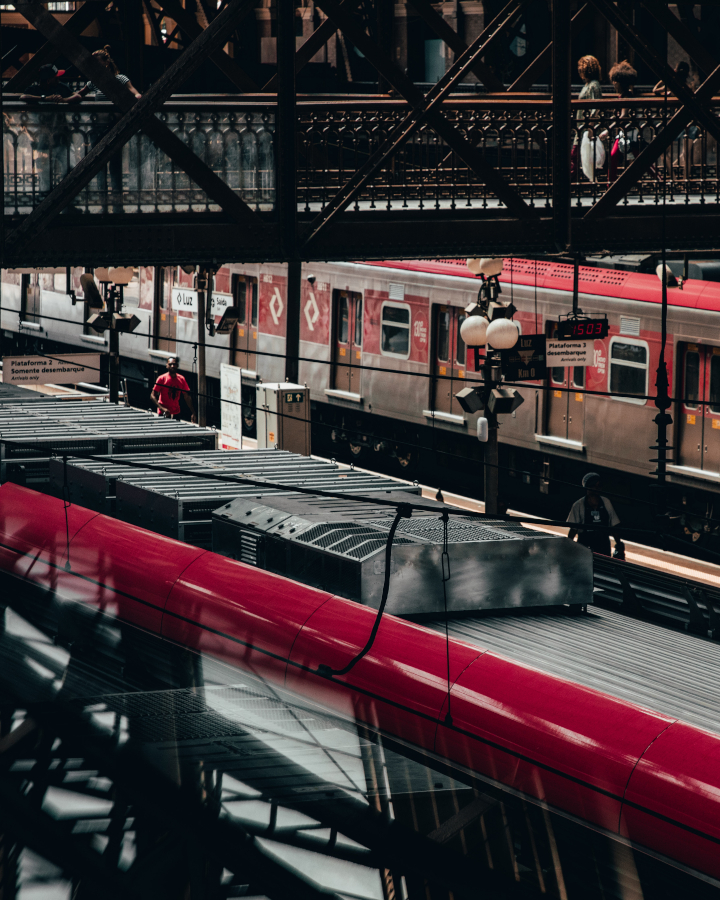
\includegraphics[scale=0.25]{estacao.eps}
    %\caption{Picture 1}
    \label{fig1:A}
  \end{subfigure}
  \begin{subfigure}[b]{0.4\textwidth}
    \includegraphics[scale=1.04]{estacao_brilho.eps}
    %\caption{Picture 2}
    \label{fig1:B}
  \end{subfigure}
\end{figure}
\setcounter{figure}{0}
\begin{figure}[h!]
  \begin{subfigure}[b]{0.5\textwidth}
    \includegraphics[scale=0.3]{estacao_rhist.eps}\\
    \includegraphics[scale=0.3]{estacao_ghist.eps}\\
    \includegraphics[scale=0.3]{estacao_bhist.eps}
    %\caption{Picture 1}
    \label{fig1:A}
  \end{subfigure}
  \begin{subfigure}[b]{0.4\textwidth}
    \includegraphics[scale=0.3]{estacao_rhist_brilho.eps}\\
    \includegraphics[scale=0.3]{estacao_ghist_brilho.eps}\\
    \includegraphics[scale=0.3]{estacao_bhist_brilho.eps}
    %\caption{Picture 2}
    \label{fig1:B}
  \end{subfigure}
  \caption{Na imagem original, à esquerda, houve um incremento no valor de 55 em
    cada pixel resultando na imagem processada.}
\end{figure}

\paragraph{}
A função \pythoninline{filtro_brilho} implementada tem como objetivo
tornar a imagem recebida como parâmetro mais clara ou escura de acordo
com o valor fornecido. Na prática ela soma/subtrai o valor de cada
pixel com limite superior em 255 e inferior em 0 dando o efeito visual
de esclarecer/escurecer a imagem.

\pagebreak

\section{Filtro de mediana}
\subsection{Código fonte}
\begin{python}
def filtro_mediana(matriz_pixels):
   altura, largura = matriz_pixels.shape[0:2]
   nova_matriz_pixels = np.zeros((altura, largura, CANAIS))
   vizinhos_canais = np.zeros((CANAIS, 8))
   for linha in range(1, altura-1):
     for coluna in range(1, largura-1):
        for cor in range(0, CANAIS):
          vizinhos_canais[cor][0] = copiar(matriz_pixels[linha-1][coluna-1][cor])
          vizinhos_canais[cor][1] = copiar(matriz_pixels[linha-1][coluna][cor])
          vizinhos_canais[cor][2] = copiar(matriz_pixels[linha-1][coluna+1][cor])
          vizinhos_canais[cor][3] = copiar(matriz_pixels[linha][coluna-1][cor])
          vizinhos_canais[cor][4] = copiar(matriz_pixels[linha][coluna+1][cor])
          vizinhos_canais[cor][5] = copiar(matriz_pixels[linha+1][coluna-1][cor])
          vizinhos_canais[cor][6] = copiar(matriz_pixels[linha+1][coluna][cor])
          vizinhos_canais[cor][7] = copiar(matriz_pixels[linha+1][coluna+1][cor])
        vizinhos_canais = np.sort(vizinhos_canais)
        nova_matriz_pixels[linha][coluna][0] = copiar(vizinhos_canais[0][3])
        nova_matriz_pixels[linha][coluna][1] = copiar(vizinhos_canais[1][3])
        nova_matriz_pixels[linha][coluna][2] = copiar(vizinhos_canais[2][3])
   return nova_matriz_pixels.astype('uint8')
\end{python}
\subsection{Exemplo de processamento}
\begin{figure}[h!]
  \begin{subfigure}[b]{0.48\textwidth}
    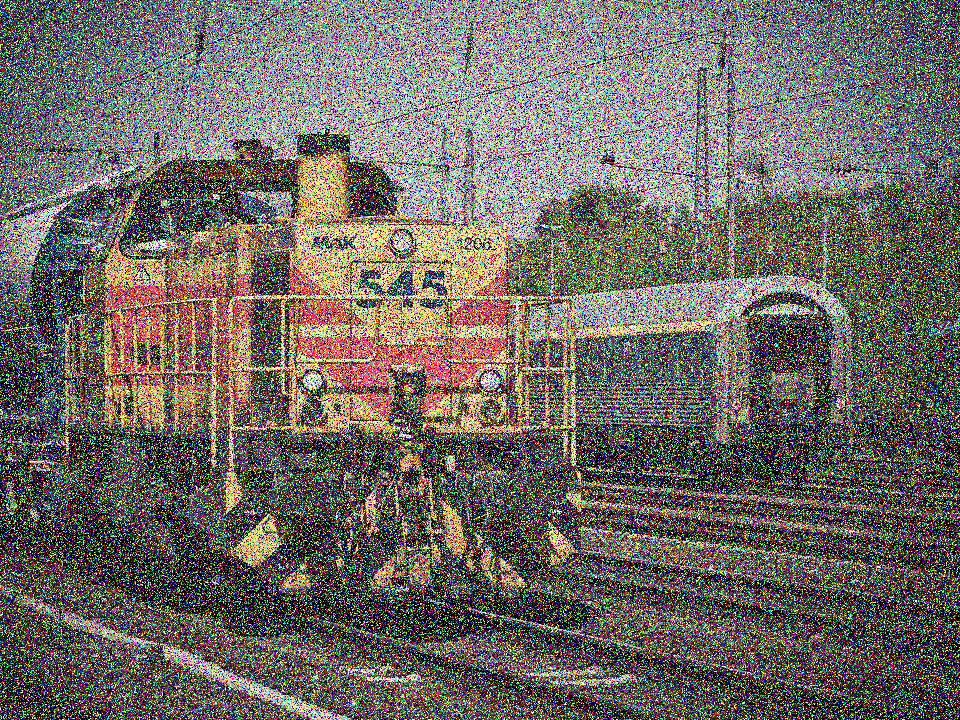
\includegraphics[scale=0.95]{ruido.eps}
    %\caption{Picture 1}
    \label{fig1:A}
  \end{subfigure}
  \begin{subfigure}[b]{0.4\textwidth}
    \includegraphics[scale=0.95]{ruido_mediana.eps}
    %\caption{Picture 2}
    \label{fig1:B}
  \end{subfigure}
\end{figure}
\setcounter{figure}{1}
\begin{figure}[h!]
  \begin{subfigure}[b]{0.5\textwidth}
    \includegraphics[scale=0.3]{ruido_rhist.eps}\\
    \includegraphics[scale=0.3]{ruido_ghist.eps}\\
    \includegraphics[scale=0.3]{ruido_bhist.eps}
    %\caption{Picture 1}
    \label{fig1:A}
  \end{subfigure}
  \begin{subfigure}[b]{0.4\textwidth}
    \includegraphics[scale=0.3]{ruido_rhist_mediana.eps}\\
    \includegraphics[scale=0.3]{ruido_ghist_mediana.eps}\\
    \includegraphics[scale=0.3]{ruido_bhist_mediana.eps}
    %\caption{Picture 2}
    \label{fig1:B}
  \end{subfigure}
  \caption{Na imagem original, à esquerda, foi aplicado o filtro de
    mediana resultando na imagem processada.}
\end{figure}

\paragraph{}
A função \pythoninline{filtro_mediana} implementada tem como objetivo
suavizar uma imagem minimizando o ruído. Na prática ela tenta remover
pixels destoantes dos seus vizinhos usando a mediana da vizinhança de
terminado pixel, removendo pontos muito intensos quando comparados ao
restante da imagem.

\pagebreak

\section{Equalização}
\subsection{Código fonte}
\begin{python}
def histograma(matriz_pixels):
   altura, largura = matriz_pixels.shape[0:2]
   histograma = np.zeros((CANAIS, VALOR_CANAL))
   for cor in range(0, CANAIS):
     for linha in range(0, altura):
       for coluna in range(0, largura):
          histograma[cor][matriz_pixels[linha][coluna][cor]] += 1
   return np.matrix(histograma)

def frequencia_acumulada(histograma):
  canais, valor_canal = histograma.shape[0:2]
  histograma_acumulado = np.zeros((canais, valor_canal))
  for cor in range(0, canais):
    histograma_acumulado[cor][0] = copiar(np.array(histograma[cor])[0][0])
    for valor_pixel in range(1, valor_canal):
      histograma_acumulado[cor][valor_pixel] =
        histograma_acumulado[cor][valor_pixel-1] + np.array(histograma[cor])[
          0][valor_pixel]
  return np.matrix(histograma_acumulado)

def filtro_equalizacao(matriz_pixels):
  nova_matriz_pixels = np.copy(matriz_pixels)
  altura, largura = nova_matriz_pixels.shape[0:2]
  numero_pixels = altura * largura
  numero_ideal_nivel = numero_pixels / (VALOR_CANAL-1)
  distribuicao_cumulativa = frequencia_acumulada(histograma(nova_matriz_pixels))
  for linha in range(0, altura):
    for coluna in range(0, largura):
      for cor in range(0, CANAIS):
        nova_matriz_pixels[linha][coluna][cor] =
          max(0, round(np.array(distribuicao_cumulativa[cor])[0][nova_matriz_pixels[
            linha][coluna][cor]] / numero_ideal_nivel)-1)
  return nova_matriz_pixels.astype('uint8')
\end{python}
\subsection{Exemplo de processamento}
\paragraph{}
A função \pythoninline{filtro_equalizacao} implementada tem como
objetivo realçar o contraste de uma imagem. Na prática ela rearranja a
distribuição de pixels de forma a buscar que cada intensidade de pixel
tenha a mesma quantidade de aparições na imagem que acaba
intensificando os detalhes.

\begin{figure}[h!]
  \begin{subfigure}[b]{0.4\textwidth}
    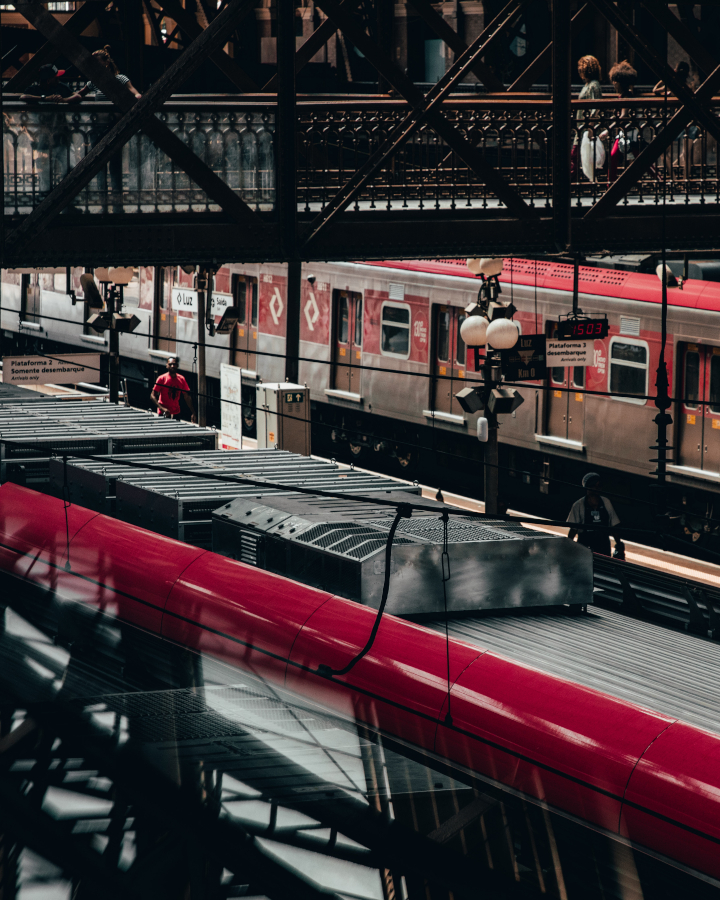
\includegraphics[scale=0.25]{estacao.eps}
    %\caption{Picture 1}
    \label{fig1:A}
  \end{subfigure}
  \begin{subfigure}[b]{0.4\textwidth}
    \includegraphics[scale=1.04]{estacao_equalizacao.eps}
    %\caption{Picture 2}
    \label{fig1:B}
  \end{subfigure}
\end{figure}
\setcounter{figure}{2}
\begin{figure}[h!]
  \begin{subfigure}[b]{0.5\textwidth}
    \includegraphics[scale=0.3]{estacao_rhist.eps}\\
    \includegraphics[scale=0.3]{estacao_ghist.eps}\\
    \includegraphics[scale=0.3]{estacao_bhist.eps}
    %\caption{Picture 1}
    \label{fig1:A}
  \end{subfigure}
  \begin{subfigure}[b]{0.4\textwidth}
    \includegraphics[scale=0.3]{estacao_rhist_equalizacao.eps}\\
    \includegraphics[scale=0.3]{estacao_ghist_equalizacao.eps}\\
    \includegraphics[scale=0.3]{estacao_bhist_equalizacao.eps}
    %\caption{Picture 2}
    \label{fig1:B}
  \end{subfigure}
  \caption{Na imagem original, à esquerda, foi aplicada a equalização
    resultando na imagem processada.}
\end{figure}

%\pagebreak

\end{document}